\begin{flushright} {\tiny {\color{gray} dgfem2D\_p1.tex}} \end{flushright}
%~~~~~~~~~~~~~~~~~~~~~~~~~~~~~~~~~~~~~~~~~~~~~~~~~~~~~~~~~~~~~~~~~~~~~~~~~~~~~~~~~~~~~~~~~~~~~~~~~~

\begin{center}
\includegraphics[width=5cm]{images/dgfem/dgelts_p1}
\end{center}

The linear basis functions in the triangle are 
\begin{eqnarray}
N_1(x,y) &=& \frac{1}{2S} ( x_2y_3-x_3y_2+(y_2-y_3)x+(x_3-x_2)y   ) \nn\\
N_2(x,y) &=& \frac{1}{2S} ( x_3y_1-x_1y_3+(y_3-y_1)x+(x_1-x_3)y   ) \nn\\
N_3(x,y) &=& \frac{1}{2S} ( x_1y_2-x_2y_1+(y_1-y_2)x+(x_2-x_1)y   ) \nn
\end{eqnarray}
where $S$ is the area of the element:
\[
S= \frac{1}{2} [(x_1-x_3)(y_2-y_3)-(x_2-x_3)(y_1-y_3)]
\]
We can easily verifiy that $N_i(x_j,y_j)=\delta_{ij}$. We then have 
\begin{eqnarray}
\partial_x N_1(x,y) &=& \frac{1}{2S}  (y_2-y_3) \nn\\
\partial_x N_2(x,y) &=& \frac{1}{2S}  (y_3-y_1) \nn\\
\partial_x N_3(x,y) &=& \frac{1}{2S}  (y_1-y_2) \nn
\end{eqnarray}
and
\begin{eqnarray}
\partial_y N_1(x,y) &=& \frac{1}{2S}  (x_3-x_2) \nn\\
\partial_y N_2(x,y) &=& \frac{1}{2S}  (x_1-x_3) \nn\\
\partial_y N_3(x,y) &=& \frac{1}{2S}  (x_2-x_1) \nn
\end{eqnarray}

Then, as shown in Section~\ref{ss:tle}, the mass matrix\footnote{The mass matrix is commonly called ${\bm M}$ 
but I use here the same notations as in Li's book.}  and the ${\bm J}_x$ and ${\bm J}_y$ matrices are:
\begin{eqnarray}
{\bm E} &=& \int_\Omega \vec{N}^T \vec{N} dV 
=\frac{S}{12} 
\left(
\begin{array}{ccc}
2 &1 &1\\ 
1 &2 &1\\
1 &1 &2
\end{array}
\right) \\
{\bm J}_x &=& - \int_{\Omega} \partial_x \vec{N}^T \vec{N}   \; dV 
=-\frac{1}{6}
\left(
\begin{array}{ccc}
y_2-y_3 & y_2-y_3 & y_2-y_3 \\
y_3-y_1 & y_3-y_1 & y_3-y_1 \\
y_1-y_2 & y_1-y_2 & y_1-y_2 
\end{array}
\right) \nn\\
{\bm J}_y &=&  - \int_{\Omega} \partial_y \vec{N}^T \vec{N}   \; dV  
=-\frac{1}{6} 
\left(
\begin{array}{ccc}
x_3-x_2 & x_3-x_2 & x_3-x_2 \\
x_1-x_3 & x_1-x_3 & x_1-x_3 \\
x_2-x_1 & x_2-x_1 & x_2-x_1 
\end{array}
\right)
\end{eqnarray}
\todo[inline]{reconcile all with minus signs}
In the same appendix we show that 
\begin{eqnarray}
{\bm C}_1 &=& \int_{\partial\Omega_3} \vec{N}^T\vec{N} dS 
= \frac{L_1}{6}
\left(
\begin{array}{ccc}
2 &1 &0\\
1 &2 &0\\
0 &0 &0
\end{array}
\right) \\ 
{\bm C}_2 &=& \int_{\partial\Omega_1} \vec{N}^T\vec{N} dS 
= \frac{L_2}{6}
\left(
\begin{array}{ccc}
0 &0 &0\\
0 &2 &1\\
0 &1 &2
\end{array}
\right) \\
{\bm C}_3 &=& \int_{\partial\Omega_2} \vec{N}^T\vec{N} dS 
= \frac{L_3}{6}
\left(
\begin{array}{ccc}
2 &0 &1\\
0 &0 &0\\
1 &0 &2
\end{array}
\right) 
\end{eqnarray}


%----------------------------------------------------------------
\subsubsection{Testing the waters - constant temperature field}

Let us assume that the temperature is constant in space. It then follows that the heat flux is identically zero. 




%----------------------------------------------------------------
\subsubsection{Testing the waters - linear temperature field}

If the temperature field is given by $T(x,y)=T_0 -a x- by$
then $q_x=a$ and $q_y=b$.







\newpage
